\section{Thesis Timeline}
We propose a thesis in five parts. Hereafter, the papers which will form the
chapters of the thesis will be referred to P1, P2, P3, P4, and P5. These are
enumerated in chronological order of submission.

The first paper, P1, detailing work already done to update DSEP to OPLIB opacity
tables and the effects those new opacity tables have on the Jao Gap location
will be submitted in the summer of 2022. The primary outstanding work for P1 
is to run population synthesis models as, observationally, the Jao Gap is
observed in populations of stars.

P2 covering self consistent modeling of NGC 2808, will be submitted sometime
between the start of the fall 2022 term and the spring 2023 term. Per Section
\ref{sec:p4} much of the background work for this paper has been completed and we are
currently ramping up modeling efforts now that we have atmospheric models in
hand. P4, consisting of modeling of both 47 Tuc and NGC 6752 will follow directly
from this work. Given P4's similarity to P2 we anticipate it will only take
three terms to submit, with an expected submission term of summer 2023.

P3 will be submitted in the spring of 2023. This paper will focus on modeling
populations of low mass stars in the local solar neighborhood in order to
determine if the location of the Jao Gap in the CMD may be used to date these
populations. Work on this paper has not yet begun. Finally, P5 will follow up
on the theoretical work from the P3; gathering archival photometric data from
low-mass stars in the local solar neighborhood and comparing Jao Gap derived
ages to ages derived from the age-velocity-dispersion relation.

These five papers, in addition to an introductory chapter, will comprise a thesis
to be defended sometime in the Summer 2024 term.

\begin{figure}
	\centering
	\definecolor{myLightGray}{RGB}{191,191,191}
\definecolor{myGray}{RGB}{160,160,160}
\definecolor{myDarkGray}{RGB}{144,144,144}
\definecolor{myDarkRed}{RGB}{167,114,115}
\definecolor{myRed}{RGB}{255,58,70}
\definecolor{myGreen}{RGB}{0,105,62}

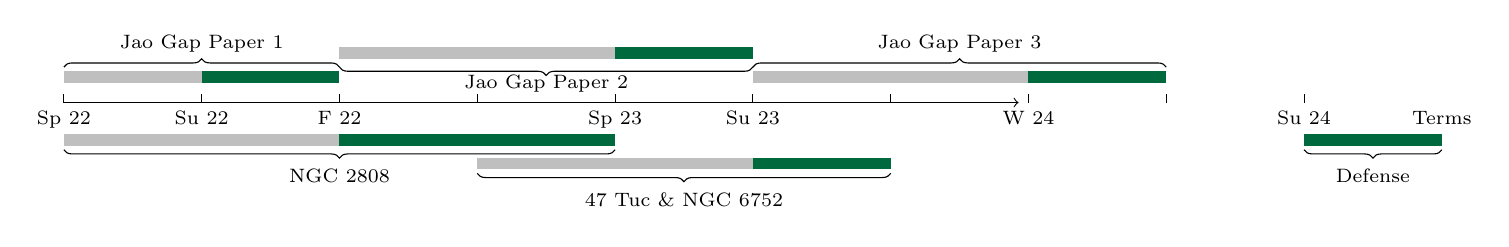
\begin{tikzpicture}[%
    every node/.style={
        font=\scriptsize,
        text height=1ex,
        text depth=.25ex,
    },
]
% draw horizontal line   
\draw[->] (0,0) -- (\textwidth,0);

% draw vertical lines
\foreach \x in {0,1,...,9}{
    \draw (1.75*\x cm,3pt) -- (1.75*\x cm,0pt);
}

% place axis labels
\node[anchor=north] at (1.75*0,0) {Sp 22};
\node[anchor=north] at (1.75*1,0) {Su 22};
\node[anchor=north] at (1.75*2,0) {F 22};
\node[anchor=north] at (1.75*4,0) {Sp 23};
\node[anchor=north] at (1.75*5,0) {Su 23};
\node[anchor=north] at (1.75*7,0) {W 24};
\node[anchor=north] at (1.75*9,0) {Su 24};
\node[anchor=north] at (1.75*10,0) {Terms};

% draw scale above
\fill[myLightGray] (1.75*0,0.25) rectangle (1.75*1,0.4);
\fill[myGreen]  (1.75*1,0.25) rectangle (1.75*2,0.4);

\fill[myLightGray] (1.75*2,0.55) rectangle (1.75*3,0.7);
\fill[myLightGray] (1.75*3,0.55) rectangle (1.75*4,0.7);
\fill[myGreen]  (1.75*4,0.55) rectangle (1.75*5,0.7);

\fill[myLightGray] (1.75*5,0.25) rectangle (1.75*6,0.4);
\fill[myLightGray] (1.75*6,0.25) rectangle (1.75*7,0.4);
\fill[myGreen]  (1.75*7,0.25) rectangle (1.75*8,0.4);
% draw scale below
\fill[myLightGray] (1.75*0,-0.4) rectangle (1.75*1,-0.55);
\fill[myLightGray] (1.75*1,-0.4) rectangle (1.75*2,-0.55);
\fill[myGreen] (1.75*2,-0.4) rectangle (1.75*3,-0.55);
\fill[myGreen] (1.75*3,-0.4) rectangle (1.75*4,-0.55);

\fill[myLightGray] (1.75*3,-0.7) rectangle (1.75*4,-0.85);
\fill[myLightGray] (1.75*4,-0.7) rectangle (1.75*5,-0.85);
\fill[myGreen] (1.75*5,-0.7) rectangle (1.75*6,-0.85);


\fill[myGreen] (1.75*9,-0.4) rectangle (1.75*10,-0.55);

% draw curly braces and add their labels
\draw[decorate,decoration={brace,amplitude=3pt}] (0,0.45) -- (1.75*2,0.45)
    node[anchor=south,midway,above=2pt] {Jao Gap Paper 1};

\draw[decorate,decoration={brace,amplitude=3pt,mirror}] (1.75*2,0.45) -- (1.75*5,0.45)
    node[anchor=north,midway,below=0pt] {Jao Gap Paper 2};

\draw[decorate,decoration={brace,amplitude=3pt}] (1.75*5,0.45) -- (1.75*8,0.45)
    node[anchor=south,midway,above=2pt] {Jao Gap Paper 3};

\draw[decorate,decoration={brace,amplitude=3pt,mirror}] (1.75*0,-0.6) -- (1.75*4,-0.6)
    node[anchor=north,midway,below=4pt] {NGC 2808};
\draw[decorate,decoration={brace,amplitude=3pt,mirror}] (1.75*3,-0.9) -- (1.75*6,-0.9)
	node[anchor=north,midway,below=4pt] {47 Tuc \& NGC 6752};

\draw[decorate,decoration={brace,amplitude=3pt,mirror}] (1.75*9,-0.6) -- (1.75*10,-0.6)
	node[anchor=north,midway,below=4pt] {Defense};

\end{tikzpicture}

	\caption{Proposed timeline for thesis work. Terms where a paper is expected
	to be submitted are marked with green, terms where work on a project is intended
	to take place are marked in grey.}
	\label{fig:timeline}
\end{figure}
